\documentclass[journal,transmag]{IEEEtran}

\usepackage{cite}
\usepackage[pdftex]{graphicx}
\graphicspath{{./Figures/}{./Charts/}}
\DeclareGraphicsExtensions{.pdf,.jpeg,.png,.jpg}
\usepackage{caption}
\usepackage{amsmath}
\interdisplaylinepenalty=2500
\usepackage{algorithmic}
\usepackage{array}
\usepackage[caption=false,font=normalsize,labelfont=sf,textfont=sf]{subfig}
\usepackage{dblfloatfix}
\usepackage{url}
\usepackage{lipsum}
\usepackage{xcolor}
\usepackage{listings}

\lstset{
	inputpath=../RayTracer/,
	escapeinside={/*@}{@*/},
	language=Java,	
	basicstyle=\fontsize{8.5}{12}\selectfont,
	numbers=left,
	numbersep=2pt,    
	xleftmargin=2pt,
	frame=tb,
	columns=fullflexible,
	showstringspaces=false,
	tabsize=4,
	keepspaces=true,
	showtabs=false,
	showspaces=false,
	morekeywords={inline,public,class,private,protected,struct},
	captionpos=b,
	lineskip=-0.4em,
	aboveskip=10pt,
	extendedchars=true,
	breaklines=true,
	prebreak = \raisebox{0ex}[0ex][0ex]{\ensuremath{\hookleftarrow}},
	keywordstyle=\color[rgb]{0,0,1},
	commentstyle=\color[rgb]{0.133,0.545,0.133},
	stringstyle=\color[rgb]{0.627,0.126,0.941},
}

% correct bad hyphenation here
\hyphenation{multi-processing}

\begin{document}

\title{An Investigation into the Speed-up of a Ray Tracer Application via the use of OpenMP and MPI}

\author{\IEEEauthorblockN{Sam Dixon \\ 40056761@live.napier.ac.uk}
\IEEEauthorblockA{SET10108 - Concurrent and Parallel Systems \\ School of Computing,
Edinburgh Napier University, Edinburgh}% <-this % stops an unwanted space

\thanks{Project available at: github.com/neaop/SET10108Coursework\_2}}


\markboth{SET10108 - Coursework 2}{}
% The only time the second header will appear is for the odd numbered pages after the title page when using the twoside option.

\IEEEtitleabstractindextext{

\begin{IEEEkeywords}
	C++11, Ray Tracer, Parallel, OpenMP, MPI, Speed-up, Efficiency
\end{IEEEkeywords}}

\maketitle

\IEEEdisplaynontitleabstractindextext

\IEEEpeerreviewmaketitle

\section{Introduction}
 
	\IEEEPARstart{T}{he} aim of this report is to document and analyse the results of an attempt to speed-up a C++11 Ray Tracer application, via the use of concurrency and parallelisation techniques. The methods being tested in this project were \texttt{OpenMP} and \texttt{MPI}.
	
	\subsection{Ray Tracing}
		Ray Tracing a rendering technique that allows an image to be generated by tracing the path of a ray as it is reflected through a virtual environment, in order to generate an accurate pixel colour on a 2D image plane. Ray Tracing aims to create photo-realistic images but the computation costs of the technique can result in significant run-times for the generation of highly detailed images. An example of how a Ray Tracer operates can be seen in Figure \ref{fig_ray_tracer_diagram}.
			
		\begin{figure}[h]
			\centering
			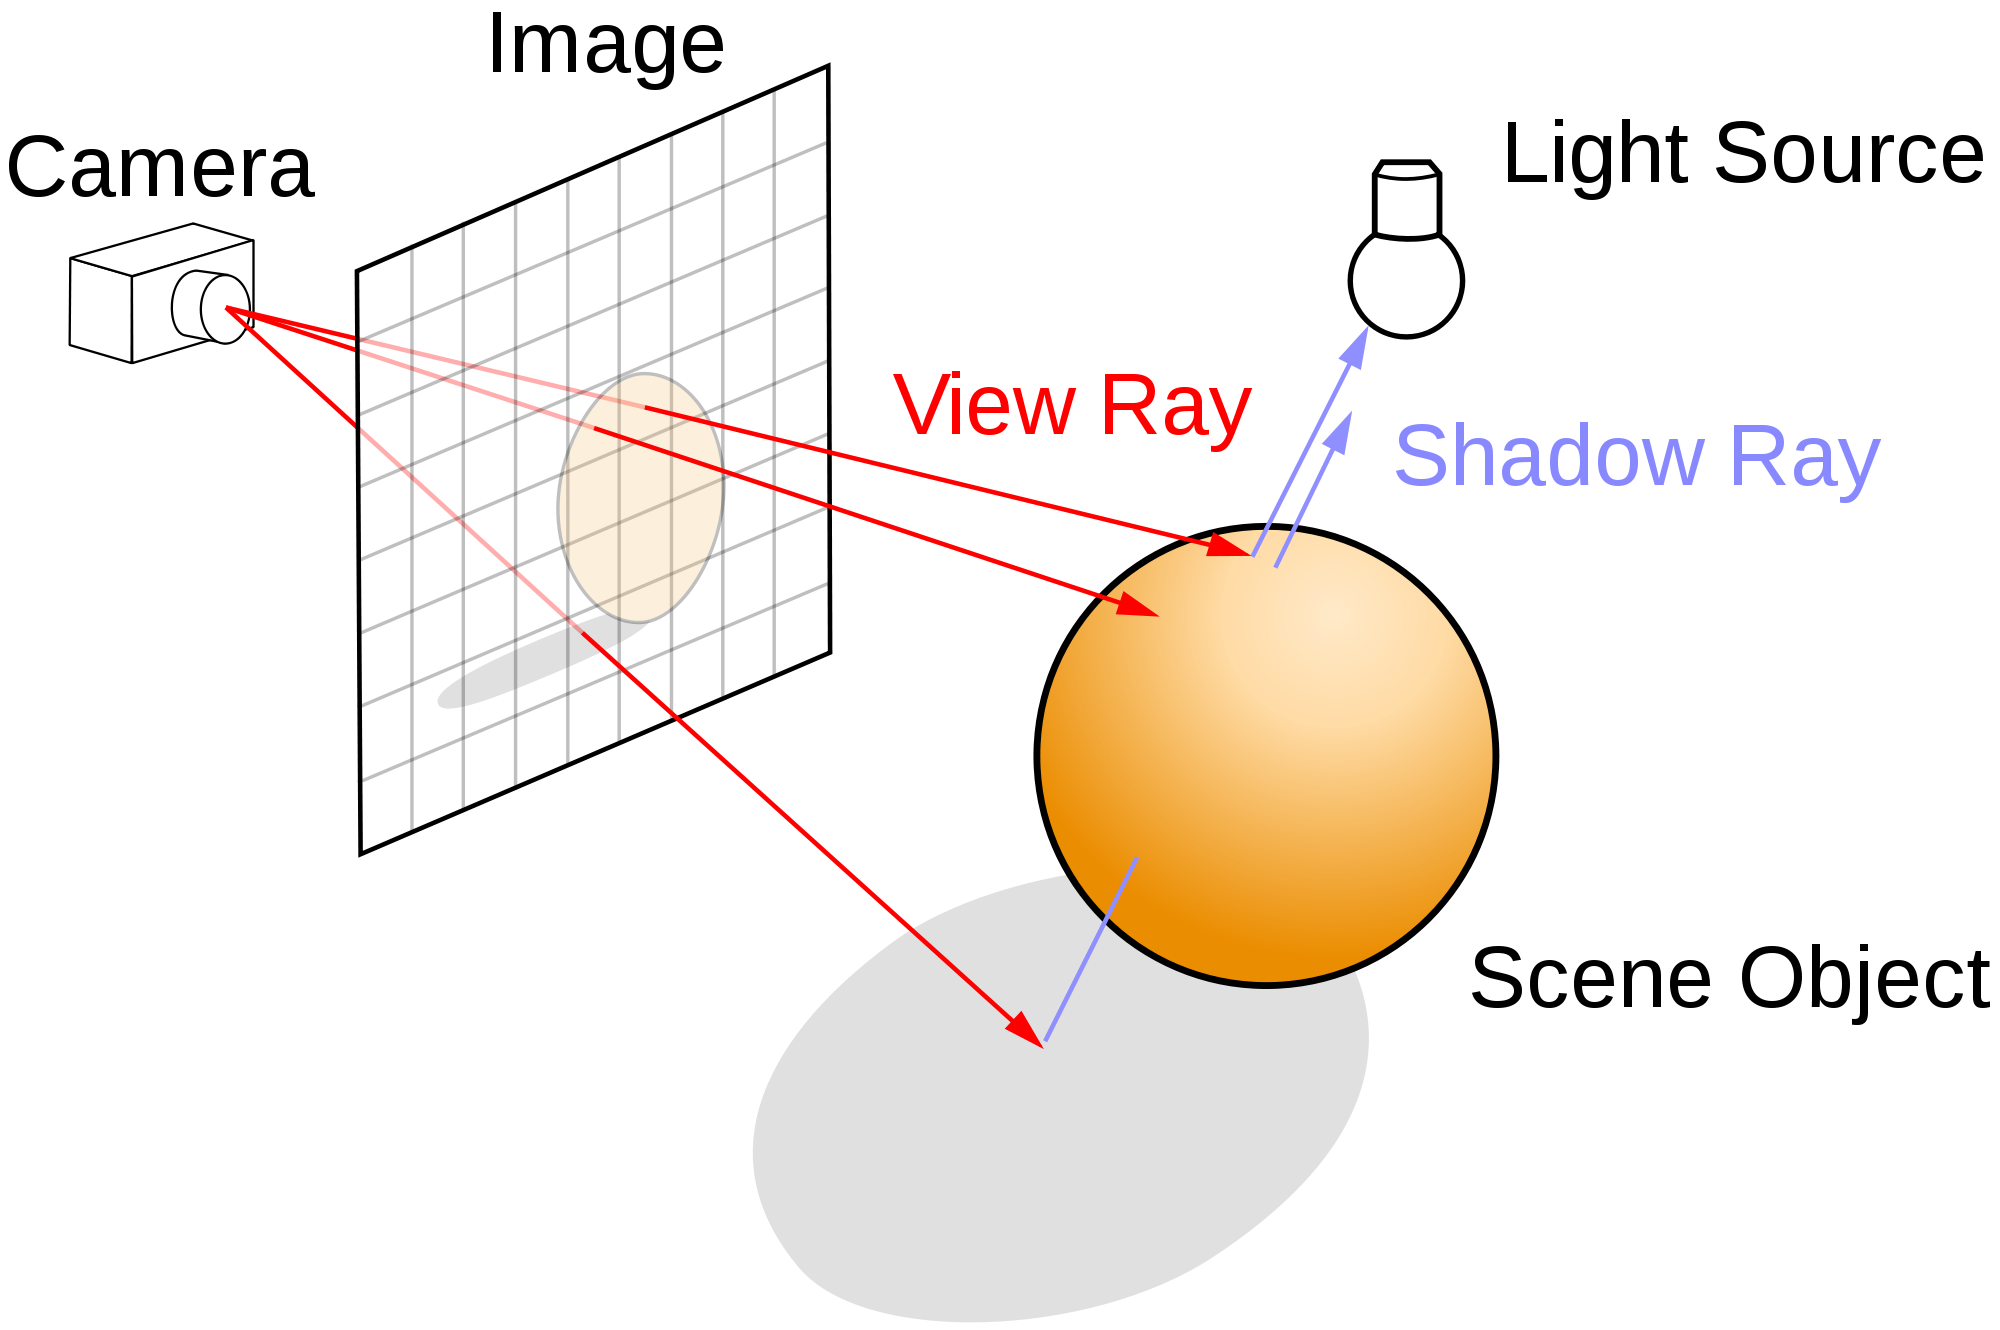
\includegraphics[width = 0.5\textwidth]{raytracerDiagram}
			\caption{A diagram of how a Ray Tracer generates an image.}
			\label{fig_ray_tracer_diagram}
		\end{figure}
	
		The Ray Tracer being analysed in this project was based on an iterative version of the \texttt{smallpt} Ray Tracer \cite{smallptG75:online}. This Ray Tracer can sample a pixel multiple times to generate a more accurate and detailed image. Two sample images are visible in Figure \ref{fig_ray_traced_images}. As can be seen - the accuracy and detail of the final images depends heavily upon the number of ray samples per pixel.
		
		Ray Tracers are ideal candidates for improvement via parallelisation techniques, as each individual ray has no dependence upon any other, thereby creating a data-parallel (or embarrassingly-parallel) problem.
		
		\begin{figure*}[]
			\centering
			\subfloat[4 Samples per Pixel]{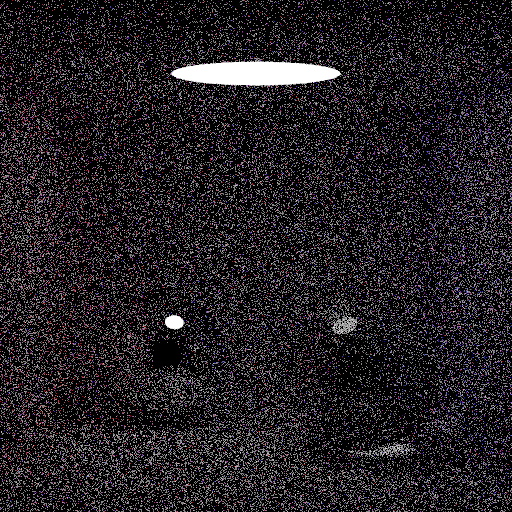
\includegraphics[width=2.5in]{raytracerSPP4}%
				\label{fig_first_image}}
			\hfil
			\subfloat[16384 Samples per Pixel]{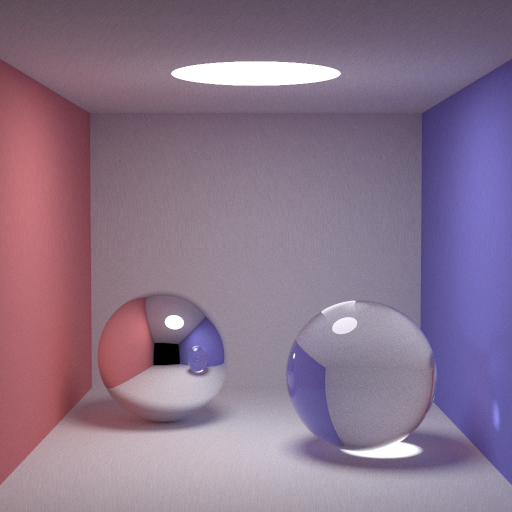
\includegraphics[width=2.5in]{raytracerSPP16384}%
				\label{fig_second_image}}
			\caption{Two images produced by the Ray Tracer.}
			\label{fig_ray_traced_images}
		\end{figure*}
		
	\subsection{OpenMP}
		\texttt{OpenMP} (Open Multi-Processing) is an open source API that allows for the implementation of shared memory multiprocessing with minimal developmental effort. \texttt{OpenMP} makes use of the C++ \texttt{\#pragma} directive and the pre-processor to allow developers to flag sections of code (particularly loops) to be parallelised. A number of different scheduling options can be implemented to alter the way in which \texttt{OpenMP} parallelises an application.
		
		The two schedulers investigated in this project are: \texttt{Static} and \texttt{Dynamic}. The \texttt{Static} scheduler will break a \texttt{for loop} into chunks, each equal to the number of iterations divided by the number of threads. E.g. in the case of a 100 iteration loop split across 4 threads: each thread would run for 25 iterations.
		
		The \texttt{Dynamic} scheduler also breaks a single \texttt{for loop} into chunks, however the chunks are typically much smaller than those produced by the \texttt{Static} scheduler. Threads are then assigned a chunk of work and upon completion can request a new chunk to work on. In this project all the dynamic chunk sizes were set to a single iteration.	

	\subsection{MPI}
		\texttt{MPI} (Message Passing Interface) is a standardised method of distributed parallelism that operates by having multiple processors communicate by sending and receiving signals from one another via communication channels. 
		
		\texttt{MPI} allows a developer to build highly scalable systems by simply providing a list of IP addresses when the application is launched. A point that developers must be aware of however is the networking overhead that distributed system innately suffer from. Figure \ref{fig_network} depicts how  the amount of time it takes to send data scales with the size of the data being sent. It should be noted that while the time taken to transfer does drop with the size of the data, eventually there is no benefit to adding more PCs to a distributed application. The full data from which the Chart was generated is visible in Appendix \ref{table_network}.

		\begin{figure}[]
			\centering
			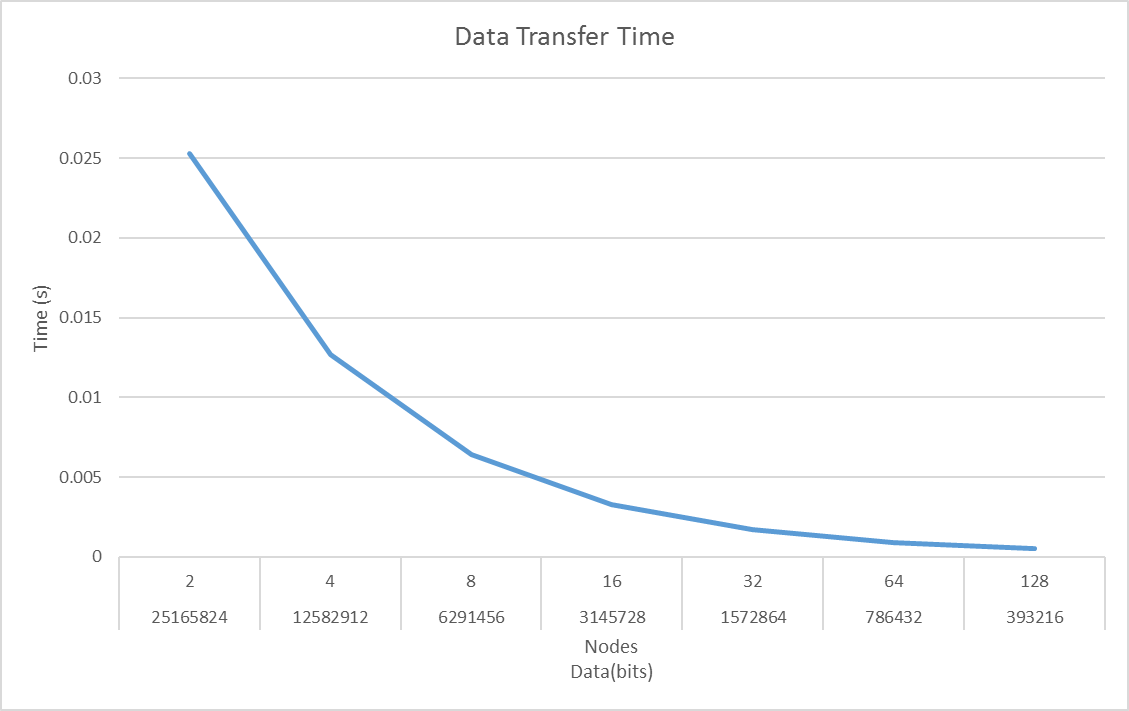
\includegraphics[width = 0.5\textwidth]{chartNetwork}
			\caption{A line chart depicting the the time required to send data over a network.}
			\label{fig_network}
		\end{figure}
		
\section{Methodology}
		
	\subsection{Profiling}
		Prior to implementing any speed-up methods, the sequential code was first analysed. By using the Visual Studio Performance Profiler, it is possible to evaluate the sequential code and locate the functions or methods that use the most CPU time. Once the potentially problematic areas have been identified, a suitable parallelisation method can be implemented to reduce the impact of those areas on the execution time. 
		
	\subsection{Data Collection}
		To ensure fair comparison and accurate results, each implementation was tested using the same parameters: Each solution produced an image 512 pixels high by 512 pixels wide, and the mean time taken for 100 attempts was recorded. This was repeated 6 times for each configuration, each time doubling the number of ray samples per pixel in order to see how each solution performed under different work loads. All benchmarking was performed on computers with the same technical specifications, which are visible in Table \ref{pcSpecsTable}. It should be noted that all code presented in the report was run without any form of compiler optimisation and that the I/O time of creating the image file is recorded in the execution time.
		
		\begin{table}[]
		\centering
		\caption{PC Specifications}
		\label{pcSpecsTable}
			\begin{tabular}{|l|l|}
				\hline
				CPU & i7-4790k 4 Core HT @ 4.00 GHz \\ \hline
				RAM & 16GB Dual Channel DDR3        \\ \hline
				GPU & Nvidia GeForce GTX 980        \\ \hline
				OS  & Windows 7 64 Bit              \\ \hline
				Bandwidth & 1 Gbit/s  				\\ \hline
				Latency   & $\sim0.12994$ ms 		\\ \hline
			\end{tabular}
		\end{table}
		
	\subsection{Evaluation}
		As well as the average execution time, speed-up and efficiency were calculated for each technique. Speed-up is defined as: 

		\[S=\frac{s_{t}}{p_{t}}\]		
		
		\noindent With \(s_{t}\) being sequential time and \(p_{t}\) being parallel time.
		Once the speed-up of a method has been calculated, the overall efficiency of the parallelisation can be measured as follows:
		
		\[E = \frac{S}{P}\]
		
		\noindent \(S\) being speed-up from the previous formula and \(P\) is the number of physical cores being utilized by the application.
		
		The two equations listed above provide standardised metrics for each method or technology tested - allowing for a fair and simple comparison of the final results.
		
\section{Implementation}
	As previously stated, the Ray Tracer presented here is a reimplementation of the iterative \texttt{smallpt} system \cite{smallptG75:online}. Several modifications had to be made to the original code to allow the implementation of parallelisation. The author of original application had written the Ray Tracer to be under 100 lines of code - which led to said code being highly obfuscated and difficult to read. Much of the development time was spent on expanding, commenting and rewriting the initial code to allow for readability and clearer functionality. One issue with the original code was the lack of smart pointers, leading to potential memory leaks. Another issue was that the program was originally designed to be compiled with \texttt{GCC}, meaning that certain methods calls were unavailable and unusable when developing within Visual Studio.
	
	\subsection{Sequential}
		Once the program was cleared up, a simple \texttt{for loop} was added to allow multiple iterations to be performed, and a file writer was used to allow the time taken for each iteration to be recorded. This sequential version of the code became the base for both the \texttt{OpenMP}, and \texttt{MPI} implementations.
	
	\subsection{OpenMP}
		Very little change had to be made to the sequential code in order to implement \texttt{OpenMP}. The most obvious location for parallelisation was the \texttt{radiance()} method, which is called from within five nested \texttt{for loop}s. By simply inserting a \texttt{\#pragma parallel for} statement above the upper-most loop, the application was made parallel, and the scheduling type and number of threads being used could be altered with very little effort.
		
	\subsection{MPI}
		A significant amount of re-basing and re-factoring had to be undertaken in order to implement \texttt{MPI} functionality within the system - not including the $\sim100$ additional lines of code. The workload of the application was split into chunks - 512 pixels wide, \(512 / number Of Nodes\) pixels high. This ensured each node was given an equally sized chunk to work on. Care also had to be taken to ensure only a single node was performing the timing and I/O operations of the system.
		
	\subsection{MPI with OpenMP}
		Similarly to the changes from the sequential to \texttt{OpenMP} code, very little of the \texttt{MPI} code had to be altered in order to include \texttt{OpenMP}. A \texttt{\#pragma parallel for} was inserted above the same the nested \texttt{for loop} as before, which allowed \texttt{MPI} nodes to create shared memory threads of there own. 
	
\section{Results}
	Data collection took a significant portion of the projects time to complete. There were $\sim198$ different parameter combinations and configurations each of which had to be run 100 times. During this time, the potential outcome of each solution could be hypothesised.
	
	\subsection{Sequential}
		The sequential code was the first to be tested, not only because it was the first configuration to be completed but also because the benchmarks produced would be used to determine the performance of the other parallelisation implementations.
		
		A chart showing the increase of execution time in regards to the number of samples per pixel is visible in Figure \ref{fig_seq_time}, and the full data in Table \ref{table_seq_data}.
		
		\begin{figure}[h]
			\centering
			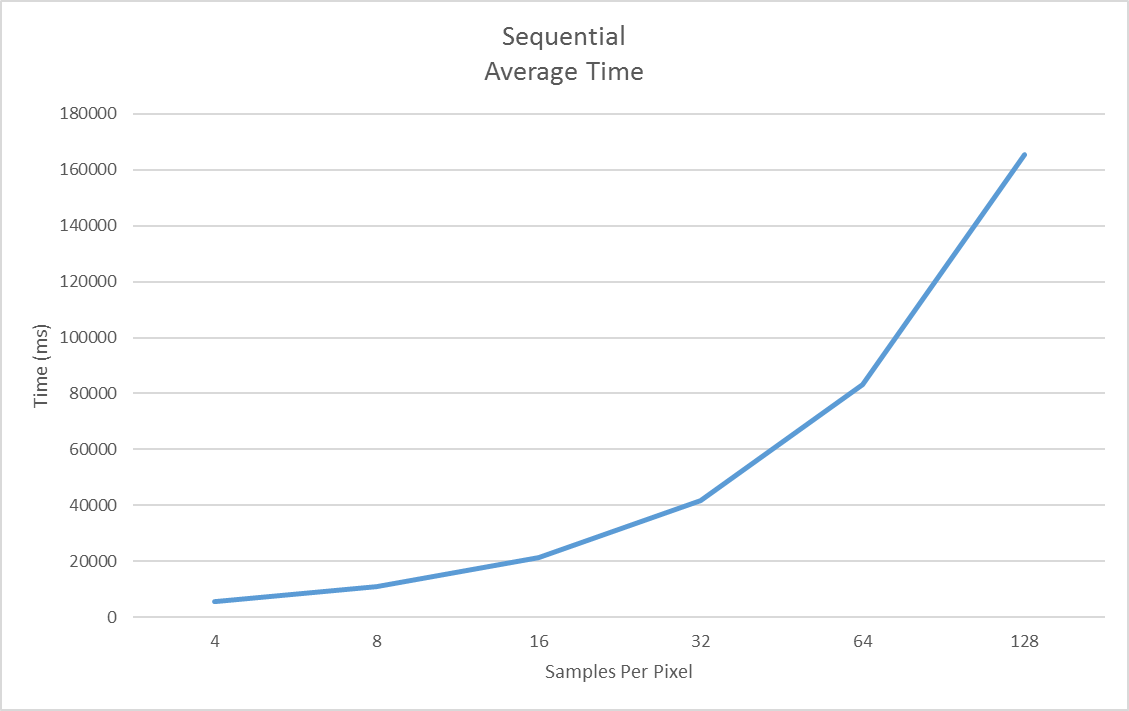
\includegraphics[width = 0.5\textwidth]{chartSeqTime}
			\caption{A line chart indicating the increase in execution time in regard to the number of colour samples per pixel.}
			\label{fig_seq_time}
		\end{figure}
	
		\begin{table}[h]
		\centering
		\caption{Sequential Benchmarks}
		\label{table_seq_data}
		\begin{tabular}{|r|r|}
			\hline
			\multicolumn{1}{|l|}{Samples} & \multicolumn{1}{l|}{Mean Time} \\ \hline
			4                             & 5735                           \\ \hline
			8                             & 10794                          \\ \hline
			16                            & 21282                          \\ \hline
			32                            & 41829                          \\ \hline
			64                            & 83256                          \\ \hline
			128                           & 165345                         \\ \hline
		\end{tabular}
	\end{table}
	
	
		

	\subsection{OpenMP}
		\subsubsection{Expected Results}
			The expected results of the \texttt{OpenMP} implementation of the ray tracer were as follows:
			Speed-up should increase with the number of threads being used, up until the hardware concurrency limit of the CPU is reached - in this case that is 8 threads.
			For efficiency, we should see an increase as the workload of each thread is incremented, as the overhead initialising a thread becomes a lower proportion of the total work being performed.
		
		\subsubsection{Actual Results}
			The speed-up and efficiency of the \texttt{OpenMP} solutions are visible in Figures \ref{fig_mpi_speed} and \ref{fig_mpi_eff}` and the raw data is available in Appendix \ref{table_omp_data}.
			
			As can be seen from the charts, the final results lined up very closely with the expected outcome. Speed-up steadily increased with the number of threads being utilized, up until 16 threads were in use. At 16 threads the number of context switches taking place on the CPU cores means there is very little benefit over simply utilizing less threads.
			
			The results for the \texttt{OpenMP} solution's efficiency followed a similar trend as the speed-up, bar the configurations that used 4 threads. The two threaded solution produced an almost linear efficiency, which would be expected as a percentage of the application must be run sequentially. It was interesting to note that both the 8 and 16 threaded configurations managed to get an efficiency of over 1 - this may be caused by some form of operating system level optimisation, or some form of specialised cache handling for applications running on multiple cores.
			
			The results also revealed that there was a slight increase in performance when utilising the \texttt{Dynamic} scheduler as opposed \texttt{Static}. This was likely due to the fact that \texttt{Dynamic} scheduling attempts to keep as many threads as possible working at once, whereas \texttt{Static} scheduling can lead to a thread completing its assigned work and then sit idle.
			
			There are number of possible reasons as to why the 4 threaded solution produced skewed results, including: Only 2 of the threads were being run on physical cores and the other 2 threads were being hyper-threaded onto the same cores, leading to unnecessary context switches. Another possible explanation for the results is that all 4 threads were being run on individual cores, but the operating system was hyper-threading background tasks onto the same cores - once again leading to unneeded context switches. 
			
		\begin{figure}[h]
			\centering
			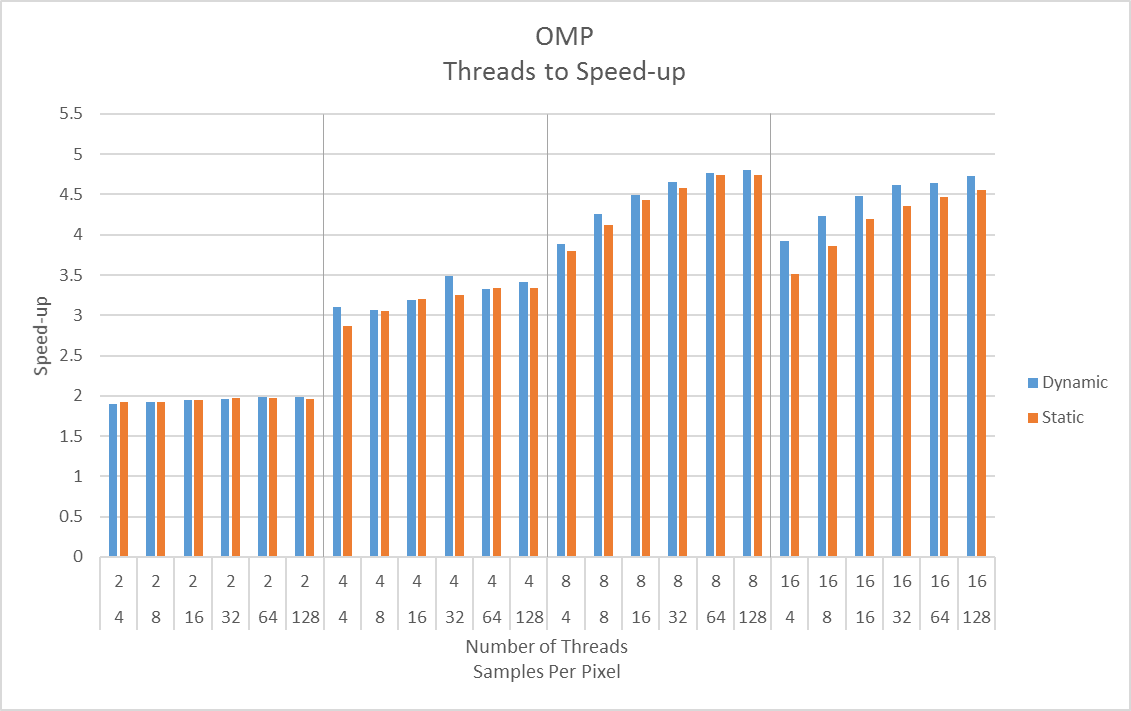
\includegraphics[width = 0.5\textwidth]{chartOMPSpeed}
			\caption{A bar chart indicating the degree of speed-up for multiple \texttt{OpenMP} schedule and thread configurations.}
			\label{fig_omp_speed}
		\end{figure}
		
		\begin{figure}[h]
			\centering
			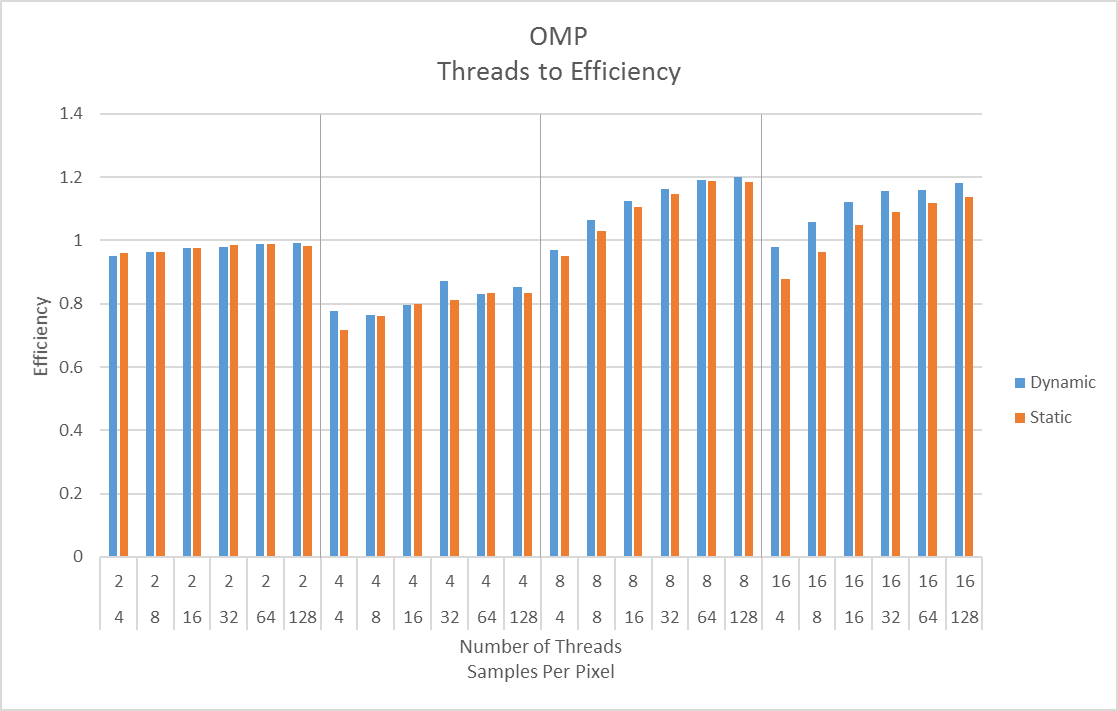
\includegraphics[width = 0.5\textwidth]{chartOMPEff}
			\caption{A bar chart indicating the degree of Efficiency for multiple \texttt{OpenMP} schedule and thread configurations.}
			\label{fig_omp_eff}
		\end{figure}
		
	\subsection{MPI}
		\subsubsection{Expected Results}
			While it was expected that \texttt{MPI} would provide a speed-up and efficiency increase over the sequential version of the algorithm - the degree of improvement was not certain, nor whether or not it would be comparable to the benefits provided by \texttt{OpenMP}.
			
			Due to the significant overheads of initialising multiple \texttt{MPI} nodes at once, the \texttt{MPI} configurations were permitted to run for an additional 10 iterations before time stamps were collected, in order to generate more consistent results and reduce outlying data points. The communication overhead of \texttt{MPI} was not considered a major bottleneck in this system, due to the specifications of network being utilized for communication.
			
		\subsubsection{Actual Results}
			In terms of speed-up (Figure \ref{fig_mpi_speed}) \texttt{MPI} provided significant benefit - reaching close to 70 times speed-up when using 16 PC's each running 8 nodes. This level of speed-up was unexpected but extremely well received. The curve of the graph also indicated that even greater speed-up could be achieved, access to additional hardware permitting.
		
			Similarly to \texttt{OpenMP}, the overall efficiency (Figure \ref{fig_mpi_eff}) of the system increases with the amount of work being done. This was mostly likely due to the initialisation overheads becoming an overall smaller percentage of the total execution time. 
			The data also reveals that using a smaller number of PC's, especially for smaller workloads, results in a higher efficiency. This demonstrates how distributed systems transition from a CPU bound problem to a I/O bound problem as the amount of hardware increases.
			
			Once again, a noticeable drop in efficiency was recorded for configurations that utilised 4 nodes. This was most likely due to the same reasons mentioned in the \texttt{OpenMP} results, but it interesting to note its occurrence across the different techniques and technologies that were tested.
			
			The full results of the \texttt{MPI} tests are visible in Appendices \ref{table_mpi_data_1} and \ref{table_mpi_data_2}.
		
		\begin{figure}[h]
			\centering
			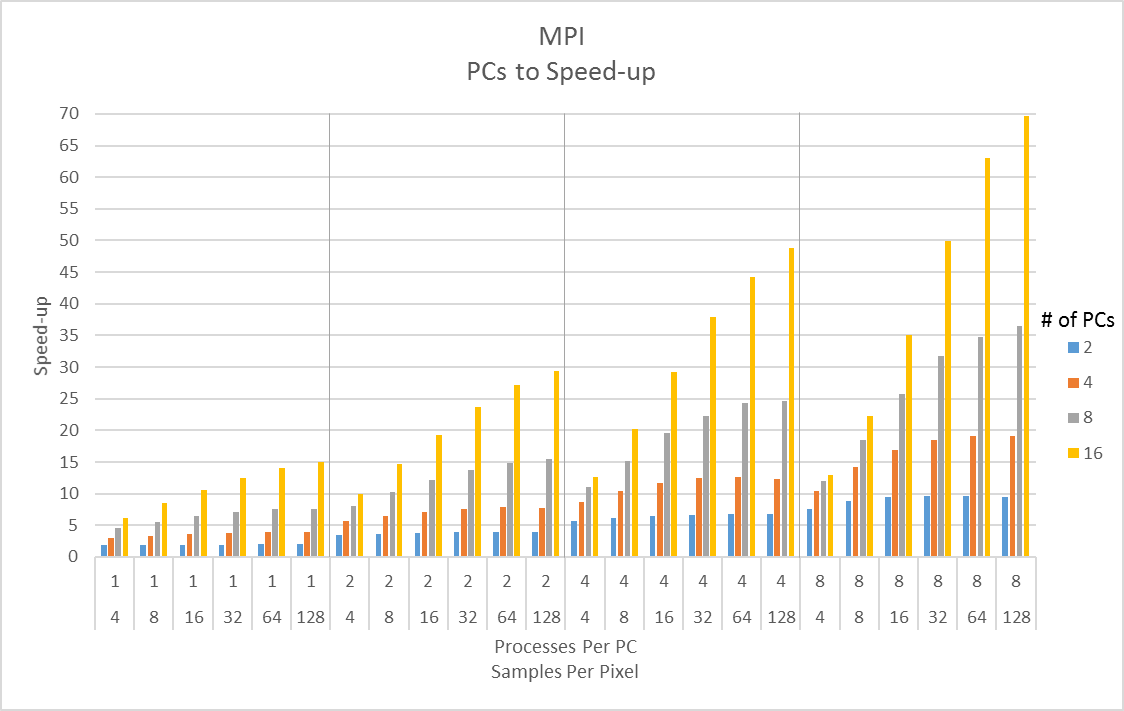
\includegraphics[width = 0.5\textwidth]{chartMPISpeed}
			\caption{A bar chart indicating the degree of speed-up for multiple \texttt{MPI} Node and Host configurations.}
			\label{fig_mpi_speed}
		\end{figure}
		
		\begin{figure}[h]
			\centering
			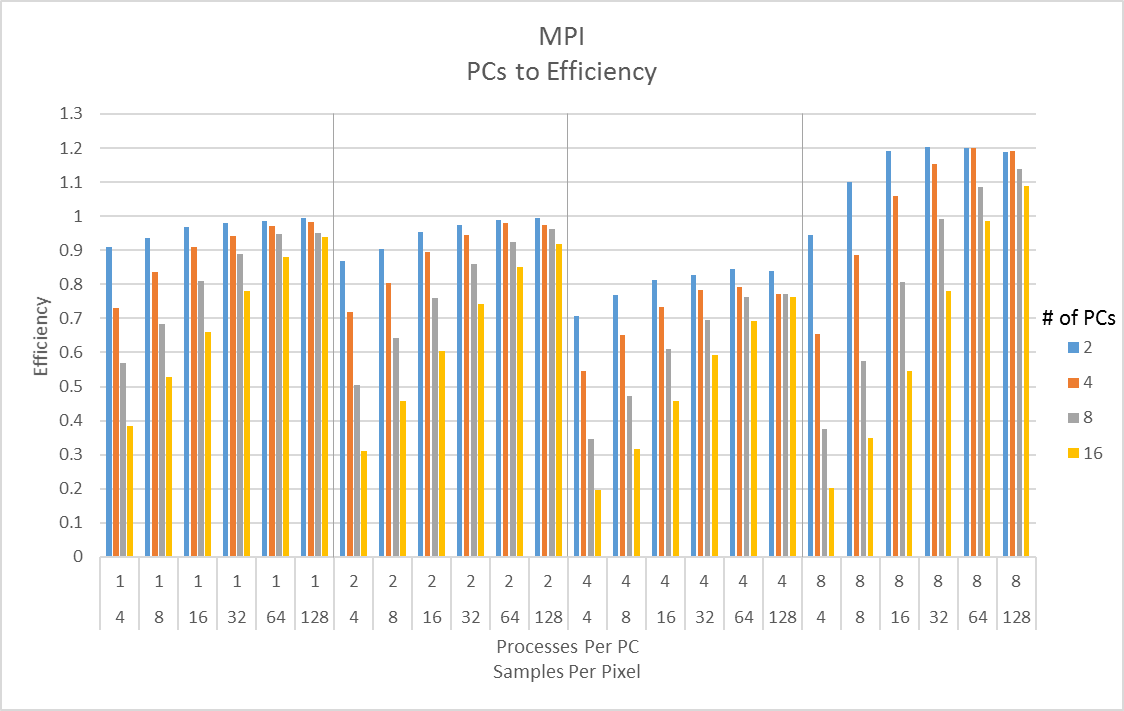
\includegraphics[width = 0.5\textwidth]{chartMPIEff}
			\caption{A bar chart indicating the degree of Efficiency for multiple \texttt{MPI} Node and Host configurations.}
			\label{fig_mpi_eff}
		\end{figure}

	\subsection{MPI with OpenMP}
		The results from the \texttt{OpenMP} tests were used to determine which configurations of \texttt{OpenMP} would be combined with \texttt{MPI} for the final implementation. Said results indicated that 8 threads offered the greatest speed-up and efficiency. For all the \texttt{MPI} with \texttt{OpenMP} tests, a single node was run on each PC and 8 \texttt{OpenMP} threads were instantiated for each of those nodes.
		 
 		\subsubsection{Expected Results}
			Similarly to the pure \texttt{MPI} implementation, the performance of the \texttt{MPI}/\texttt{OpenMP} solution was uncertain. It was believed that the combined solution would produce overall the better results, but the degree of those could not be ascertained.
		
		\subsubsection{Actual Results}
			For speed-up, Figure \ref{fig_ompi_speed}, the curve of results was very similar to that witnessed on the pure \texttt{MPI} solution, Figure \ref{fig_mpi_speed}. The only major difference between the two graphs being the level of speed-up, with the combined solution loosing $\sim12\%$ when compared to pure \texttt{MPI}. This was particularly interesting, as it was hypothesised that \texttt{MPI} with \texttt{OpenMP} would produce faster results, but it appears that the combined overhead of the technologies was more of a hindrance than a benefit.
			
			Regarding efficiency, Figure \ref{fig_ompi_eff}, there is not much to say that has not already been said about the pure \texttt{MPI} version. The overall efficiency of the system drops as the number of PCs in the system increases - again this likely due to problem transitioning from CPU boundaries to I/O boundaries.
			
			It is worth noting that neither \texttt{Static} or \texttt{Dynamic} scheduling produced significantly different results. This was likely due to the workload of each individual thread being very small - the total workload was already split between each PC and then further divided for each \texttt{OpenMP} thread.
			
		\begin{figure}[h]
			\centering
			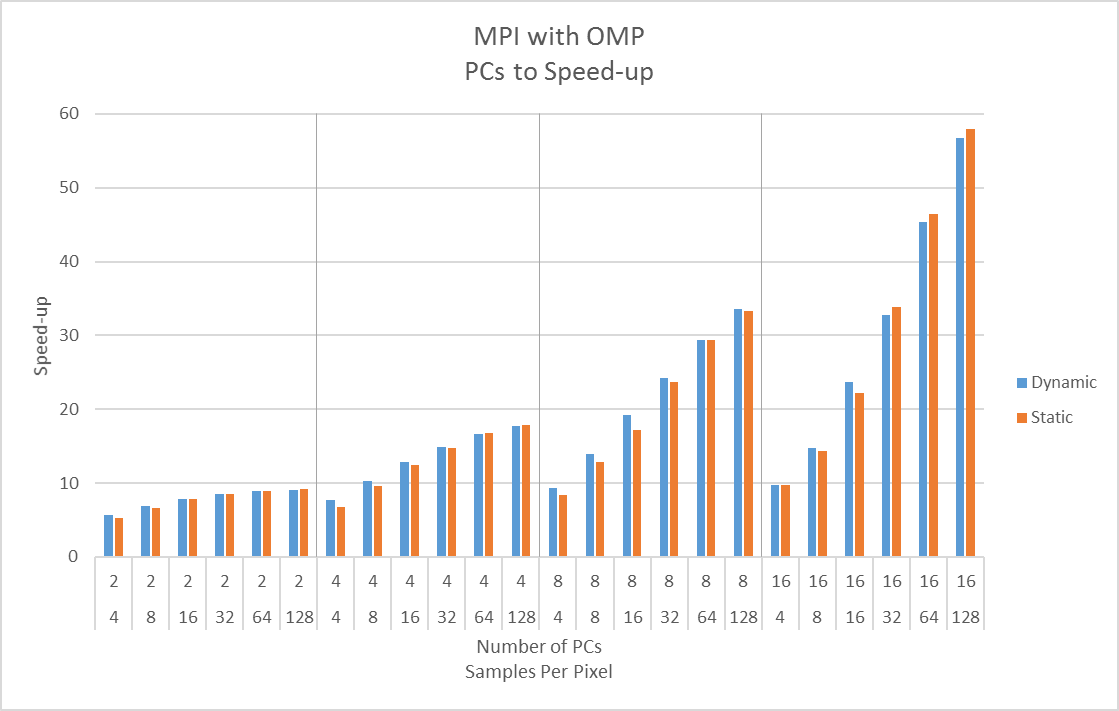
\includegraphics[width = 0.5\textwidth]{chartOMPISpeed}
			\caption{A bar chart indicating the degree of speed-up when using \texttt{MPI} and \texttt{OpenMP} with various scheduling types and number of Hosts configurations.}
			\label{fig_ompi_speed}
		\end{figure}
		
		\begin{figure}[h]
			\centering
			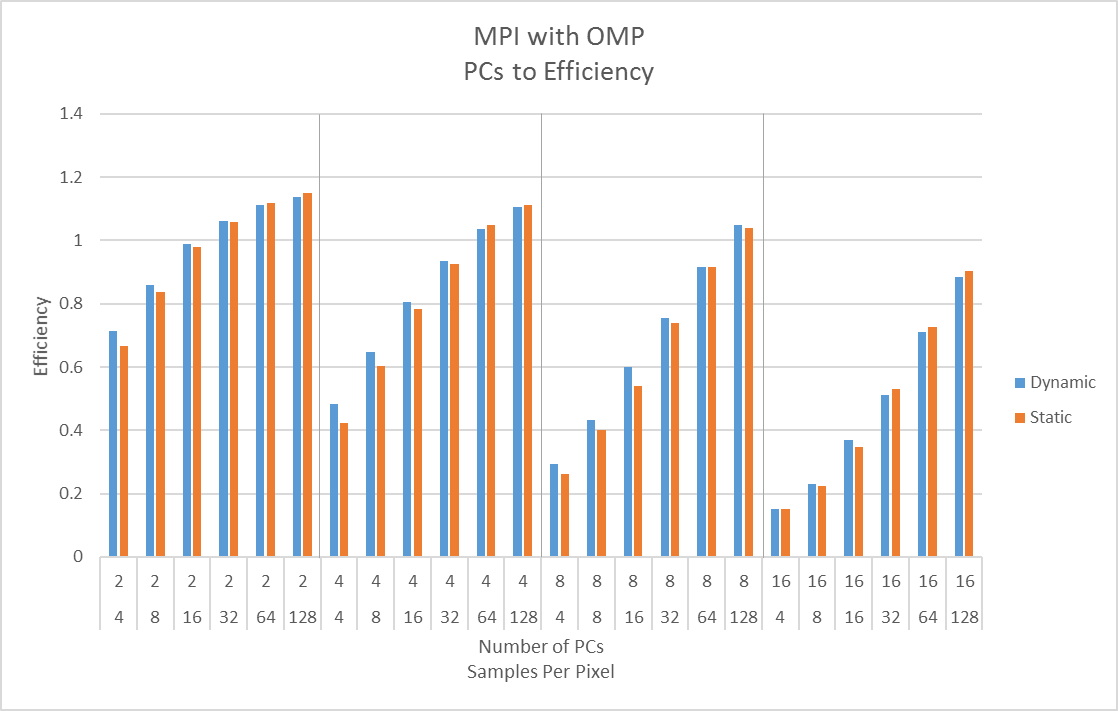
\includegraphics[width = 0.5\textwidth]{chartOMPIEff}
			\caption{A bar chart indicating the degree of Efficiency when using \texttt{MPI} and \texttt{OpenMP} with various scheduling types and number of Hosts configurations.}
			\label{fig_ompi_eff}
		\end{figure}

	
\section{Conclusion}
	An excessive and exhaustive amount of testing and analysis led to a final result: For this particular application, pure \texttt{MPI} provided greater speed-up and efficiency than pure \texttt{OpenMP}, or a combined implementation of both technologies. While this result is well received, there still exists potential for further future work: testing the \texttt{MPI} implementations on even larger numbers of PCs, examining what effects compiler optimisation can have on performance and looking into sequential code optimisations further reduce the execution time of the program.
	 
	\subsection{Reflection}
	Having very little experience with distributed systems, this project came with a great many challenges and frustrations - but the final result of a fully functional, and exceptional fast Ray Tracer outshone the frustrations of working with \texttt{MPI}, \texttt{C++} and a very sparsely commented code base.

\bibliographystyle{IEEEtran}
\bibliography{Bibliography}
%\nocite{Williams:1483005}

\newpage
\onecolumn
\appendices

\section{}
\begin{figure}[h]
	\centering
	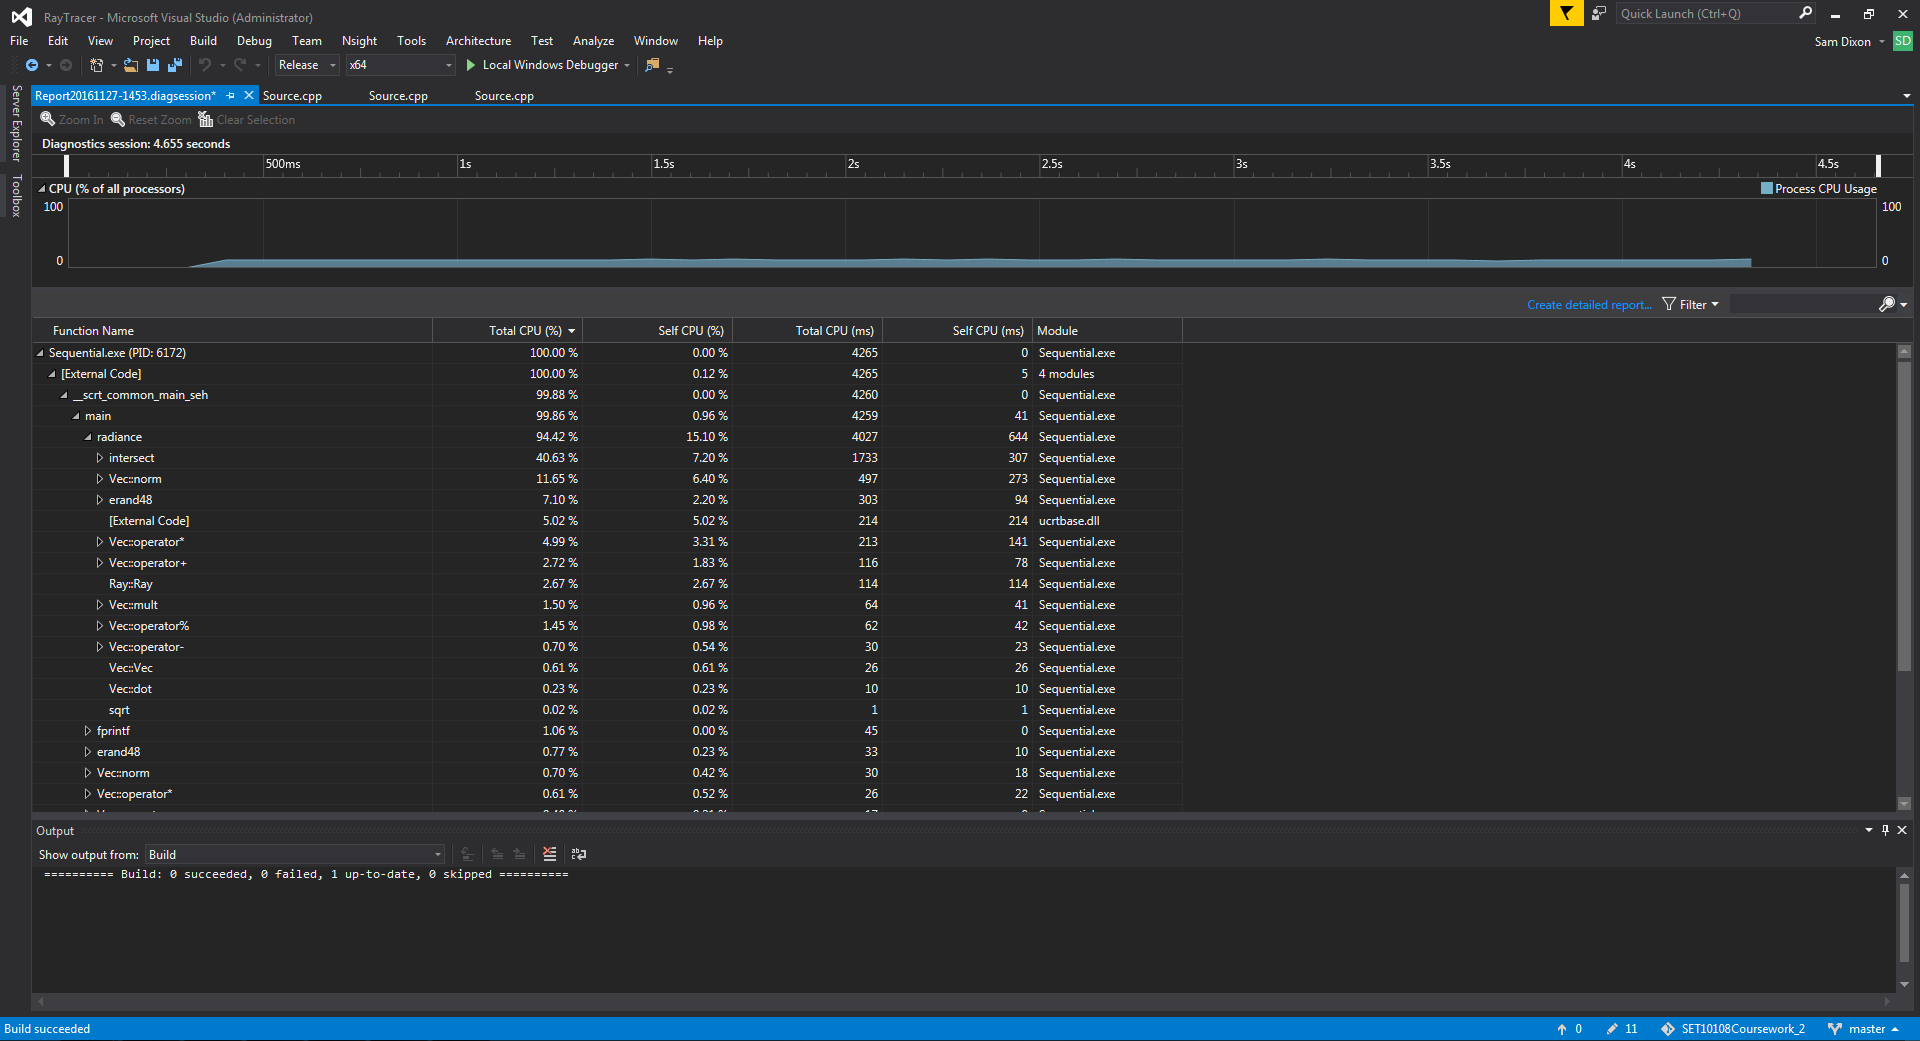
\includegraphics[width =\textwidth]{sequentialProfile}
	\caption{The Visual Studio code profile of the sequential implementation of the ray tracer.}
	\label{fig_seq_prfile}
\end{figure}

\section{}
\begin{table*}[h]
	\centering
	\caption{Data transfer times over a network.}
	\label{table_network}
	\begin{tabular}{|r|r|r|r|r|r|r|r|r|r|}
		\hline
		\multicolumn{1}{|l|}{Nodes} & \multicolumn{1}{l|}{Width} & \multicolumn{1}{l|}{Height} & \multicolumn{1}{l|}{Chunk Size} & \multicolumn{1}{l|}{Pixels Per Node} & \multicolumn{1}{l|}{Vec size (bits)} & \multicolumn{1}{l|}{Total Data (bits)} & \multicolumn{1}{l|}{Bandwidth bits/s} & \multicolumn{1}{l|}{Latency(s)} & \multicolumn{1}{l|}{Time (s)} \\ \hline
		2                           & 512                        & 512                         & 256                             & 131072                               & 192                                  & 25165824                               & 1000000000                            & 0.00013                         & 0.02530                       \\ \hline
		4                           & 512                        & 512                         & 128                             & 65536                                & 192                                  & 12582912                               & 1000000000                            & 0.00013                         & 0.01271                       \\ \hline
		8                           & 512                        & 512                         & 64                              & 32768                                & 192                                  & 6291456                                & 1000000000                            & 0.00013                         & 0.00642                       \\ \hline
		16                          & 512                        & 512                         & 32                              & 16384                                & 192                                  & 3145728                                & 1000000000                            & 0.00013                         & 0.00328                       \\ \hline
		32                          & 512                        & 512                         & 16                              & 8192                                 & 192                                  & 1572864                                & 1000000000                            & 0.00013                         & 0.00170                       \\ \hline
		64                          & 512                        & 512                         & 8                               & 4096                                 & 192                                  & 786432                                 & 1000000000                            & 0.00013                         & 0.00092                       \\ \hline
		128                         & 512                        & 512                         & 4                               & 2048                                 & 192                                  & 393216                                 & 1000000000                            & 0.00013                         & 0.00052                       \\ \hline
	\end{tabular}
\end{table*}

	\newpage
	
\section{}
	\begin{table*}[h]		
	\centering
	\caption{OMP Speed-up and Efficiency}
	\label{table_omp_data}
	\begin{tabular}{|l|r|r|r|r|r|}
		\hline
		Schedule & \multicolumn{1}{l|}{Samples} & \multicolumn{1}{l|}{Threads} & \multicolumn{1}{l|}{Mean Time} & \multicolumn{1}{l|}{Speed-up} & \multicolumn{1}{l|}{Efficiency} \\ \hline
		Dynamic       & 4                            & 2                            & 3014                              & 1.90279                       & 0.95139                         \\ \hline
		Dynamic       & 8                            & 2                            & 5600                              & 1.92750                       & 0.96375                         \\ \hline
		Dynamic       & 16                           & 2                            & 10895                             & 1.95337                       & 0.97669                         \\ \hline
		Dynamic       & 32                           & 2                            & 21389                             & 1.95563                       & 0.97782                         \\ \hline
		Dynamic       & 64                           & 2                            & 42033                             & 1.98073                       & 0.99036                         \\ \hline
		Dynamic       & 128                          & 2                            & 83384                             & 1.98293                       & 0.99147                         \\ \hline
		Dynamic       & 4                            & 4                            & 1848                              & 3.10335                       & 0.77584                         \\ \hline
		Dynamic       & 8                            & 4                            & 3525                              & 3.06213                       & 0.76553                         \\ \hline
		Dynamic       & 16                           & 4                            & 6684                              & 3.18402                       & 0.79601                         \\ \hline
		Dynamic       & 32                           & 4                            & 11987                             & 3.48953                       & 0.87238                         \\ \hline
		Dynamic       & 64                           & 4                            & 25062                             & 3.32200                       & 0.83050                         \\ \hline
		Dynamic       & 128                          & 4                            & 48495                             & 3.40953                       & 0.85238                         \\ \hline
		Dynamic       & 4                            & 8                            & 1477                              & 3.88287                       & 0.97072                         \\ \hline
		Dynamic       & 8                            & 8                            & 2538                              & 4.25296                       & 1.06324                         \\ \hline
		Dynamic       & 16                           & 8                            & 4731                              & 4.49841                       & 1.12460                         \\ \hline
		Dynamic       & 32                           & 8                            & 8998                              & 4.64870                       & 1.16217                         \\ \hline
		Dynamic       & 64                           & 8                            & 17454                             & 4.77002                       & 1.19251                         \\ \hline
		Dynamic       & 128                          & 8                            & 34447                             & 4.79998                       & 1.20000                         \\ \hline
		Dynamic       & 4                            & 16                           & 1463                              & 3.92003                       & 0.98001                         \\ \hline
		Dynamic       & 8                            & 16                           & 2551                              & 4.23128                       & 1.05782                         \\ \hline
		Dynamic       & 16                           & 16                           & 4749                              & 4.48136                       & 1.12034                         \\ \hline
		Dynamic       & 32                           & 16                           & 9054                              & 4.61995                       & 1.15499                         \\ \hline
		Dynamic       & 64                           & 16                           & 17938                             & 4.64132                       & 1.16033                         \\ \hline
		Dynamic       & 128                          & 16                           & 34953                             & 4.73050                       & 1.18262                         \\ \hline
		Static        & 4                            & 2                            & 2987                              & 1.91999                       & 0.95999                         \\ \hline
		Static        & 8                            & 2                            & 5604                              & 1.92612                       & 0.96306                         \\ \hline
		Static        & 16                           & 2                            & 10903                             & 1.95194                       & 0.97597                         \\ \hline
		Static        & 32                           & 2                            & 21237                             & 1.96963                       & 0.98481                         \\ \hline
		Static        & 64                           & 2                            & 42101                             & 1.97753                       & 0.98877                         \\ \hline
		Static        & 128                          & 2                            & 84127                             & 1.96542                       & 0.98271                         \\ \hline
		Static        & 4                            & 4                            & 1999                              & 2.86893                       & 0.71723                         \\ \hline
		Static        & 8                            & 4                            & 3538                              & 3.05088                       & 0.76272                         \\ \hline
		Static        & 16                           & 4                            & 6654                              & 3.19838                       & 0.79959                         \\ \hline
		Static        & 32                           & 4                            & 12881                             & 3.24734                       & 0.81184                         \\ \hline
		Static        & 64                           & 4                            & 24933                             & 3.33919                       & 0.83480                         \\ \hline
		Static        & 128                          & 4                            & 49619                             & 3.33229                       & 0.83307                         \\ \hline
		Static        & 4                            & 8                            & 1508                              & 3.80305                       & 0.95076                         \\ \hline
		Static        & 8                            & 8                            & 2621                              & 4.11828                       & 1.02957                         \\ \hline
		Static        & 16                           & 8                            & 4806                              & 4.42821                       & 1.10705                         \\ \hline
		Static        & 32                           & 8                            & 9130                              & 4.58149                       & 1.14537                         \\ \hline
		Static        & 64                           & 8                            & 17541                             & 4.74637                       & 1.18659                         \\ \hline
		Static        & 128                          & 8                            & 34886                             & 4.73958                       & 1.18490                         \\ \hline
		Static        & 4                            & 16                           & 1631                              & 3.51625                       & 0.87906                         \\ \hline
		Static        & 8                            & 16                           & 2799                              & 3.85638                       & 0.96409                         \\ \hline
		Static        & 16                           & 16                           & 5073                              & 4.19515                       & 1.04879                         \\ \hline
		Static        & 32                           & 16                           & 9606                              & 4.35447                       & 1.08862                         \\ \hline
		Static        & 64                           & 16                           & 18609                             & 4.47396                       & 1.11849                         \\ \hline
		Static        & 128                          & 16                           & 36336                             & 4.55045                       & 1.13761                         \\ \hline
	\end{tabular}
\end{table*}
	\newpage
	
\section{}
	\begin{table*}[h]
	\centering
	\caption{MPI Speed-up and Efficiency (Part 1)}
	\label{table_mpi_data_1}
	\begin{tabular}{|r|r|r|r|r|r|}
		\hline
		\multicolumn{1}{|l|}{Samples} & \multicolumn{1}{l|}{Hosts} & \multicolumn{1}{l|}{Nodes} & \multicolumn{1}{l|}{Mean Time} & \multicolumn{1}{l|}{Speed-up} & \multicolumn{1}{l|}{Efficiency} \\ \hline
		4                             & 2                          & 2                                & 3150                           & 1.82063                       & 0.91032                         \\ \hline
		8                             & 2                          & 2                                & 5762                           & 1.87331                       & 0.93665                         \\ \hline
		16                            & 2                          & 2                                & 11001                          & 1.93455                       & 0.96728                         \\ \hline
		32                            & 2                          & 2                                & 21369                          & 1.95746                       & 0.97873                         \\ \hline
		64                            & 2                          & 2                                & 42198                          & 1.97298                       & 0.98649                         \\ \hline
		128                           & 2                          & 2                                & 83011                          & 1.99184                       & 0.99592                         \\ \hline
		4                             & 2                          & 4                                & 1651                           & 3.47365                       & 0.86841                         \\ \hline
		8                             & 2                          & 4                                & 2982                           & 3.61972                       & 0.90493                         \\ \hline
		16                            & 2                          & 4                                & 5578                           & 3.81535                       & 0.95384                         \\ \hline
		32                            & 2                          & 4                                & 10724                          & 3.90050                       & 0.97513                         \\ \hline
		64                            & 2                          & 4                                & 21024                          & 3.96005                       & 0.99001                         \\ \hline
		128                           & 2                          & 4                                & 41535                          & 3.98086                       & 0.99521                         \\ \hline
		4                             & 2                          & 8                                & 1012                           & 5.66700                       & 0.70837                         \\ \hline
		8                             & 2                          & 8                                & 1758                           & 6.13993                       & 0.76749                         \\ \hline
		16                            & 2                          & 8                                & 3277                           & 6.49435                       & 0.81179                         \\ \hline
		32                            & 2                          & 8                                & 6312                           & 6.62690                       & 0.82836                         \\ \hline
		64                            & 2                          & 8                                & 12331                          & 6.75176                       & 0.84397                         \\ \hline
		128                           & 2                          & 8                                & 24648                          & 6.70825                       & 0.83853                         \\ \hline
		4                             & 2                          & 16                               & 759                            & 7.55599                       & 0.94450                         \\ \hline
		8                             & 2                          & 16                               & 1225                           & 8.81143                       & 1.10143                         \\ \hline
		16                            & 2                          & 16                               & 2232                           & 9.53495                       & 1.19187                         \\ \hline
		32                            & 2                          & 16                               & 4343                           & 9.63136                       & 1.20392                         \\ \hline
		64                            & 2                          & 16                               & 8684                           & 9.58729                       & 1.19841                         \\ \hline
		128                           & 2                          & 16                               & 17395                          & 9.50532                       & 1.18816                         \\ \hline
		4                             & 4                          & 4                                & 1959                           & 2.92751                       & 0.73188                         \\ \hline
		8                             & 4                          & 4                                & 3224                           & 3.34801                       & 0.83700                         \\ \hline
		16                            & 4                          & 4                                & 5856                           & 3.63422                       & 0.90856                         \\ \hline
		32                            & 4                          & 4                                & 11096                          & 3.76974                       & 0.94243                         \\ \hline
		64                            & 4                          & 4                                & 21441                          & 3.88303                       & 0.97076                         \\ \hline
		128                           & 4                          & 4                                & 42075                          & 3.92977                       & 0.98244                         \\ \hline
		4                             & 4                          & 8                                & 999                            & 5.74074                       & 0.71759                         \\ \hline
		8                             & 4                          & 8                                & 1681                           & 6.42118                       & 0.80265                         \\ \hline
		16                            & 4                          & 8                                & 2971                           & 7.16324                       & 0.89541                         \\ \hline
		32                            & 4                          & 8                                & 5533                           & 7.55991                       & 0.94499                         \\ \hline
		64                            & 4                          & 8                                & 10622                          & 7.83807                       & 0.97976                         \\ \hline
		128                           & 4                          & 8                                & 21225                          & 7.79011                       & 0.97376                         \\ \hline
		4                             & 4                          & 16                               & 656                            & 8.74238                       & 0.54640                         \\ \hline
		8                             & 4                          & 16                               & 1038                           & 10.39884                      & 0.64993                         \\ \hline
		16                            & 4                          & 16                               & 1812                           & 11.74503                      & 0.73406                         \\ \hline
		32                            & 4                          & 16                               & 3344                           & 12.50867                      & 0.78179                         \\ \hline
		64                            & 4                          & 16                               & 6569                           & 12.67408                      & 0.79213                         \\ \hline
		128                           & 4                          & 16                               & 13404                          & 12.33550                      & 0.77097                         \\ \hline
		4                             & 4                          & 32                               & 549                            & 10.44627                      & 0.65289                         \\ \hline
		8                             & 4                          & 32                               & 762                            & 14.16535                      & 0.88533                         \\ \hline
		16                            & 4                          & 32                               & 1257                           & 16.93079                      & 1.05817                         \\ \hline
		32                            & 4                          & 32                               & 2265                           & 18.46755                      & 1.15422                         \\ \hline
		64                            & 4                          & 32                               & 4340                           & 19.18341                      & 1.19896                         \\ \hline
		128                           & 4                          & 32                               & 8681                           & 19.04677                      & 1.19042                         \\ \hline
	\end{tabular}
\end{table*}
	\newpage
	
\section{}
	\begin{table*}[h]
	\centering
	\caption{MPI Speed-up and Efficiency (Part 2)}
	\label{table_mpi_data_2}
	\begin{tabular}{|r|r|r|r|r|r|}
		\hline
		\multicolumn{1}{|l|}{Samples} & \multicolumn{1}{l|}{Hosts} & \multicolumn{1}{l|}{Nodes} & \multicolumn{1}{l|}{Mean Time} & \multicolumn{1}{l|}{Speed-up} & \multicolumn{1}{l|}{Efficiency} \\ \hline
		4                             & 8                          & 8                                & 1259                           & 4.55520                       & 0.56940                         \\ \hline
		8                             & 8                          & 8                                & 1971                           & 5.47641                       & 0.68455                         \\ \hline
		16                            & 8                          & 8                                & 3286                           & 6.47657                       & 0.80957                         \\ \hline
		32                            & 8                          & 8                                & 5881                           & 7.11257                       & 0.88907                         \\ \hline
		64                            & 8                          & 8                                & 10988                          & 7.57699                       & 0.94712                         \\ \hline
		128                           & 8                          & 8                                & 21727                          & 7.61012                       & 0.95126                         \\ \hline
		4                             & 8                          & 16                               & 710                            & 8.07746                       & 0.50484                         \\ \hline
		8                             & 8                          & 16                               & 1049                           & 10.28980                      & 0.64311                         \\ \hline
		16                            & 8                          & 16                               & 1753                           & 12.14033                      & 0.75877                         \\ \hline
		32                            & 8                          & 16                               & 3037                           & 13.77313                      & 0.86082                         \\ \hline
		64                            & 8                          & 16                               & 5633                           & 14.78005                      & 0.92375                         \\ \hline
		128                           & 8                          & 16                               & 10734                          & 15.40386                      & 0.96274                         \\ \hline
		4                             & 8                          & 32                               & 518                            & 11.07143                      & 0.34598                         \\ \hline
		8                             & 8                          & 32                               & 714                            & 15.11765                      & 0.47243                         \\ \hline
		16                            & 8                          & 32                               & 1091                           & 19.50687                      & 0.60959                         \\ \hline
		32                            & 8                          & 32                               & 1882                           & 22.22582                      & 0.69456                         \\ \hline
		64                            & 8                          & 32                               & 3417                           & 24.36523                      & 0.76141                         \\ \hline
		128                           & 8                          & 32                               & 6691                           & 24.71155                      & 0.77224                         \\ \hline
		4                             & 8                          & 64                               & 477                            & 12.02306                      & 0.37572                         \\ \hline
		8                             & 8                          & 64                               & 586                            & 18.41980                      & 0.57562                         \\ \hline
		16                            & 8                          & 64                               & 825                            & 25.79636                      & 0.80614                         \\ \hline
		32                            & 8                          & 64                               & 1320                           & 31.68864                      & 0.99027                         \\ \hline
		64                            & 8                          & 64                               & 2397                           & 34.73342                      & 1.08542                         \\ \hline
		128                           & 8                          & 64                               & 4535                           & 36.45976                      & 1.13937                         \\ \hline
		4                             & 16                         & 16                               & 934                            & 6.14026                       & 0.38377                         \\ \hline
		8                             & 16                         & 16                               & 1278                           & 8.44601                       & 0.52788                         \\ \hline
		16                            & 16                         & 16                               & 2012                           & 10.57753                      & 0.66110                         \\ \hline
		32                            & 16                         & 16                               & 3352                           & 12.47882                      & 0.77993                         \\ \hline
		64                            & 16                         & 16                               & 5921                           & 14.06114                      & 0.87882                         \\ \hline
		128                           & 16                         & 16                               & 10997                          & 15.03546                      & 0.93972                         \\ \hline
		4                             & 16                         & 32                               & 579                            & 9.90501                       & 0.30953                         \\ \hline
		8                             & 16                         & 32                               & 735                            & 14.68571                      & 0.45893                         \\ \hline
		16                            & 16                         & 32                               & 1103                           & 19.29465                      & 0.60296                         \\ \hline
		32                            & 16                         & 32                               & 1762                           & 23.73950                      & 0.74186                         \\ \hline
		64                            & 16                         & 32                               & 3063                           & 27.18119                      & 0.84941                         \\ \hline
		128                           & 16                         & 32                               & 5619                           & 29.42605                      & 0.91956                         \\ \hline
		4                             & 16                         & 64                               & 453                            & 12.66004                      & 0.19781                         \\ \hline
		8                             & 16                         & 64                               & 535                            & 20.17570                      & 0.31525                         \\ \hline
		16                            & 16                         & 64                               & 728                            & 29.23352                      & 0.45677                         \\ \hline
		32                            & 16                         & 64                               & 1104                           & 37.88859                      & 0.59201                         \\ \hline
		64                            & 16                         & 64                               & 1883                           & 44.21455                      & 0.69085                         \\ \hline
		128                           & 16                         & 64                               & 3393                           & 48.73121                      & 0.76143                         \\ \hline
		4                             & 16                         & 128                              & 441                            & 13.00454                      & 0.20320                         \\ \hline
		8                             & 16                         & 128                              & 484                            & 22.30165                      & 0.34846                         \\ \hline
		16                            & 16                         & 128                              & 608                            & 35.00329                      & 0.54693                         \\ \hline
		32                            & 16                         & 128                              & 837                            & 49.97491                      & 0.78086                         \\ \hline
		64                            & 16                         & 128                              & 1320                           & 63.07273                      & 0.98551                         \\ \hline
		128                           & 16                         & 128                              & 2376                           & 69.58965                      & 1.08734                         \\ \hline
	\end{tabular}
\end{table*}
	\newpage
	
\section{}
	\begin{table*}[h]
	\centering
	\caption{MPI with OMP Speed-up and Efficiency}
	\label{table_ompi_data}
	\begin{tabular}{|r|l|r|r|r|r|r|}
		\hline
		\multicolumn{1}{|l|}{Samples} & Schedule & \multicolumn{1}{l|}{Hosts} & \multicolumn{1}{l|}{Nodes} & \multicolumn{1}{l|}{Mean Time} & \multicolumn{1}{l|}{Speed-up} & \multicolumn{1}{l|}{Efficiency} \\ \hline
		4                             & Dynamic  & 2                          & 2                          & 1002                           & 5.72355                       & 0.71544                         \\ \hline
		8                             & Dynamic  & 2                          & 2                          & 1572                           & 6.86641                       & 0.85830                         \\ \hline
		16                            & Dynamic  & 2                          & 2                          & 2694                           & 7.89978                       & 0.98747                         \\ \hline
		32                            & Dynamic  & 2                          & 2                          & 4927                           & 8.48975                       & 1.06122                         \\ \hline
		64                            & Dynamic  & 2                          & 2                          & 9367                           & 8.88822                       & 1.11103                         \\ \hline
		128                           & Dynamic  & 2                          & 2                          & 18150                          & 9.10992                       & 1.13874                         \\ \hline
		4                             & Dynamic  & 4                          & 4                          & 744                            & 7.70833                       & 0.48177                         \\ \hline
		8                             & Dynamic  & 4                          & 4                          & 1044                           & 10.33908                      & 0.64619                         \\ \hline
		16                            & Dynamic  & 4                          & 4                          & 1652                           & 12.88257                      & 0.80516                         \\ \hline
		32                            & Dynamic  & 4                          & 4                          & 2797                           & 14.95495                      & 0.93468                         \\ \hline
		64                            & Dynamic  & 4                          & 4                          & 5014                           & 16.60471                      & 1.03779                         \\ \hline
		128                           & Dynamic  & 4                          & 4                          & 9351                           & 17.68207                      & 1.10513                         \\ \hline
		4                             & Dynamic  & 8                          & 8                          & 610                            & 9.40164                       & 0.29380                         \\ \hline
		8                             & Dynamic  & 8                          & 8                          & 778                            & 13.87404                      & 0.43356                         \\ \hline
		16                            & Dynamic  & 8                          & 8                          & 1111                           & 19.15572                      & 0.59862                         \\ \hline
		32                            & Dynamic  & 8                          & 8                          & 1729                           & 24.19260                      & 0.75602                         \\ \hline
		64                            & Dynamic  & 8                          & 8                          & 2840                           & 29.31549                      & 0.91611                         \\ \hline
		128                           & Dynamic  & 8                          & 8                          & 4925                           & 33.57259                      & 1.04914                         \\ \hline
		4                             & Dynamic  & 16                         & 16                         & 591                            & 9.70389                       & 0.15162                         \\ \hline
		8                             & Dynamic  & 16                         & 16                         & 734                            & 14.70572                      & 0.22978                         \\ \hline
		16                            & Dynamic  & 16                         & 16                         & 898                            & 23.69933                      & 0.37030                         \\ \hline
		32                            & Dynamic  & 16                         & 16                         & 1278                           & 32.73005                      & 0.51141                         \\ \hline
		64                            & Dynamic  & 16                         & 16                         & 1834                           & 45.39586                      & 0.70931                         \\ \hline
		128                           & Dynamic  & 16                         & 16                         & 2917                           & 56.68324                      & 0.88568                         \\ \hline
		4                             & Static   & 2                          & 2                          & 1077                           & 5.32498                       & 0.66562                         \\ \hline
		8                             & Static   & 2                          & 2                          & 1613                           & 6.69188                       & 0.83648                         \\ \hline
		16                            & Static   & 2                          & 2                          & 2716                           & 7.83579                       & 0.97947                         \\ \hline
		32                            & Static   & 2                          & 2                          & 4937                           & 8.47255                       & 1.05907                         \\ \hline
		64                            & Static   & 2                          & 2                          & 9297                           & 8.95515                       & 1.11939                         \\ \hline
		128                           & Static   & 2                          & 2                          & 17986                          & 9.19298                       & 1.14912                         \\ \hline
		4                             & Static   & 4                          & 4                          & 845                            & 6.78698                       & 0.42419                         \\ \hline
		8                             & Static   & 4                          & 4                          & 1116                           & 9.67204                       & 0.60450                         \\ \hline
		16                            & Static   & 4                          & 4                          & 1701                           & 12.51146                      & 0.78197                         \\ \hline
		32                            & Static   & 4                          & 4                          & 2825                           & 14.80673                      & 0.92542                         \\ \hline
		64                            & Static   & 4                          & 4                          & 4963                           & 16.77534                      & 1.04846                         \\ \hline
		128                           & Static   & 4                          & 4                          & 9288                           & 17.80200                      & 1.11263                         \\ \hline
		4                             & Static   & 8                          & 8                          & 682                            & 8.40909                       & 0.26278                         \\ \hline
		8                             & Static   & 8                          & 8                          & 844                            & 12.78910                      & 0.39966                         \\ \hline
		16                            & Static   & 8                          & 8                          & 1234                           & 17.24635                      & 0.53895                         \\ \hline
		32                            & Static   & 8                          & 8                          & 1770                           & 23.63220                      & 0.73851                         \\ \hline
		64                            & Static   & 8                          & 8                          & 2837                           & 29.34649                      & 0.91708                         \\ \hline
		128                           & Static   & 8                          & 8                          & 4973                           & 33.24854                      & 1.03902                         \\ \hline
		4                             & Static   & 16                         & 16                         & 587                            & 9.77002                       & 0.15266                         \\ \hline
		8                             & Static   & 16                         & 16                         & 751                            & 14.37284                      & 0.22458                         \\ \hline
		16                            & Static   & 16                         & 16                         & 956                            & 22.26151                      & 0.34784                         \\ \hline
		32                            & Static   & 16                         & 16                         & 1234                           & 33.89708                      & 0.52964                         \\ \hline
		64                            & Static   & 16                         & 16                         & 1793                           & 46.43391                      & 0.72553                         \\ \hline
		128                           & Static   & 16                         & 16                         & 2855                           & 57.91419                      & 0.90491                         \\ \hline
	\end{tabular}
\end{table*}
	\newpage
	


\end{document}